\section{The Circuit: Vanilla model of a Discrete Time Crystal}


\begin{figure}[h]
\begin{subfigure}{0.59\textwidth}
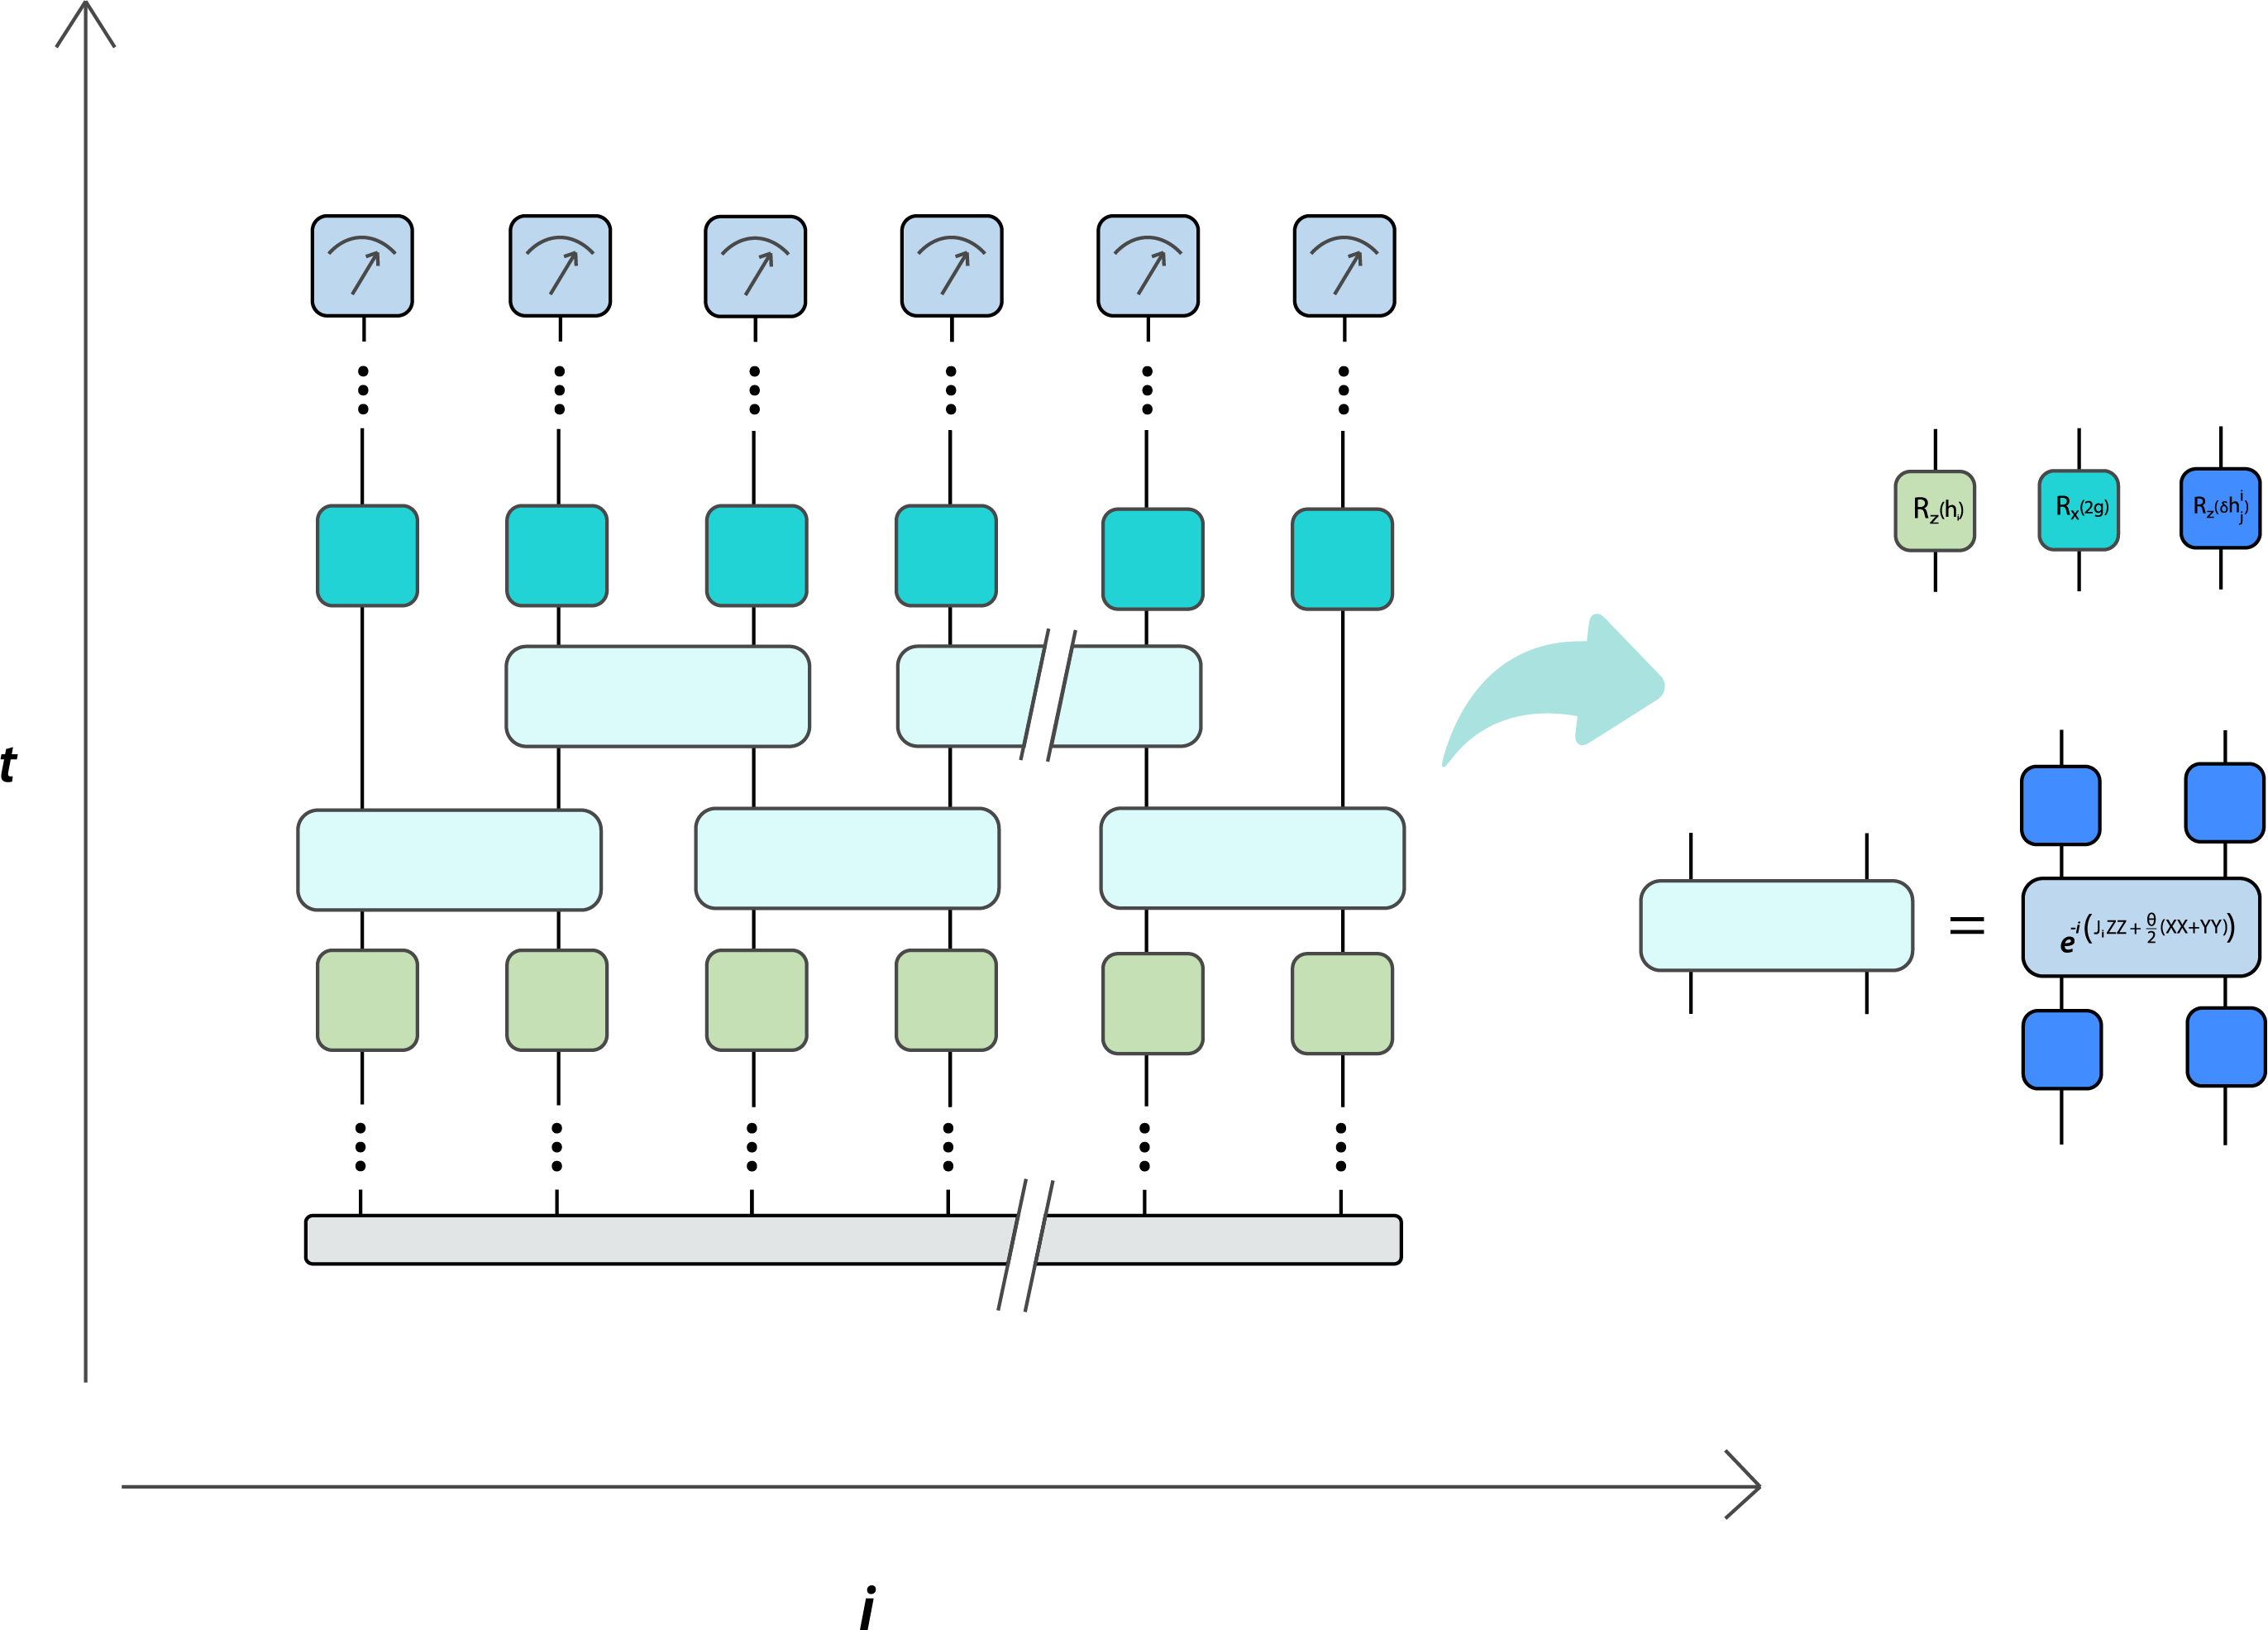
\includegraphics[width=0.9\linewidth]{.src/images/DTC/model/DTC circuit.png} 
\label{fig:DTC-circuit}
\end{subfigure}
\begin{subfigure}{0.39\textwidth}
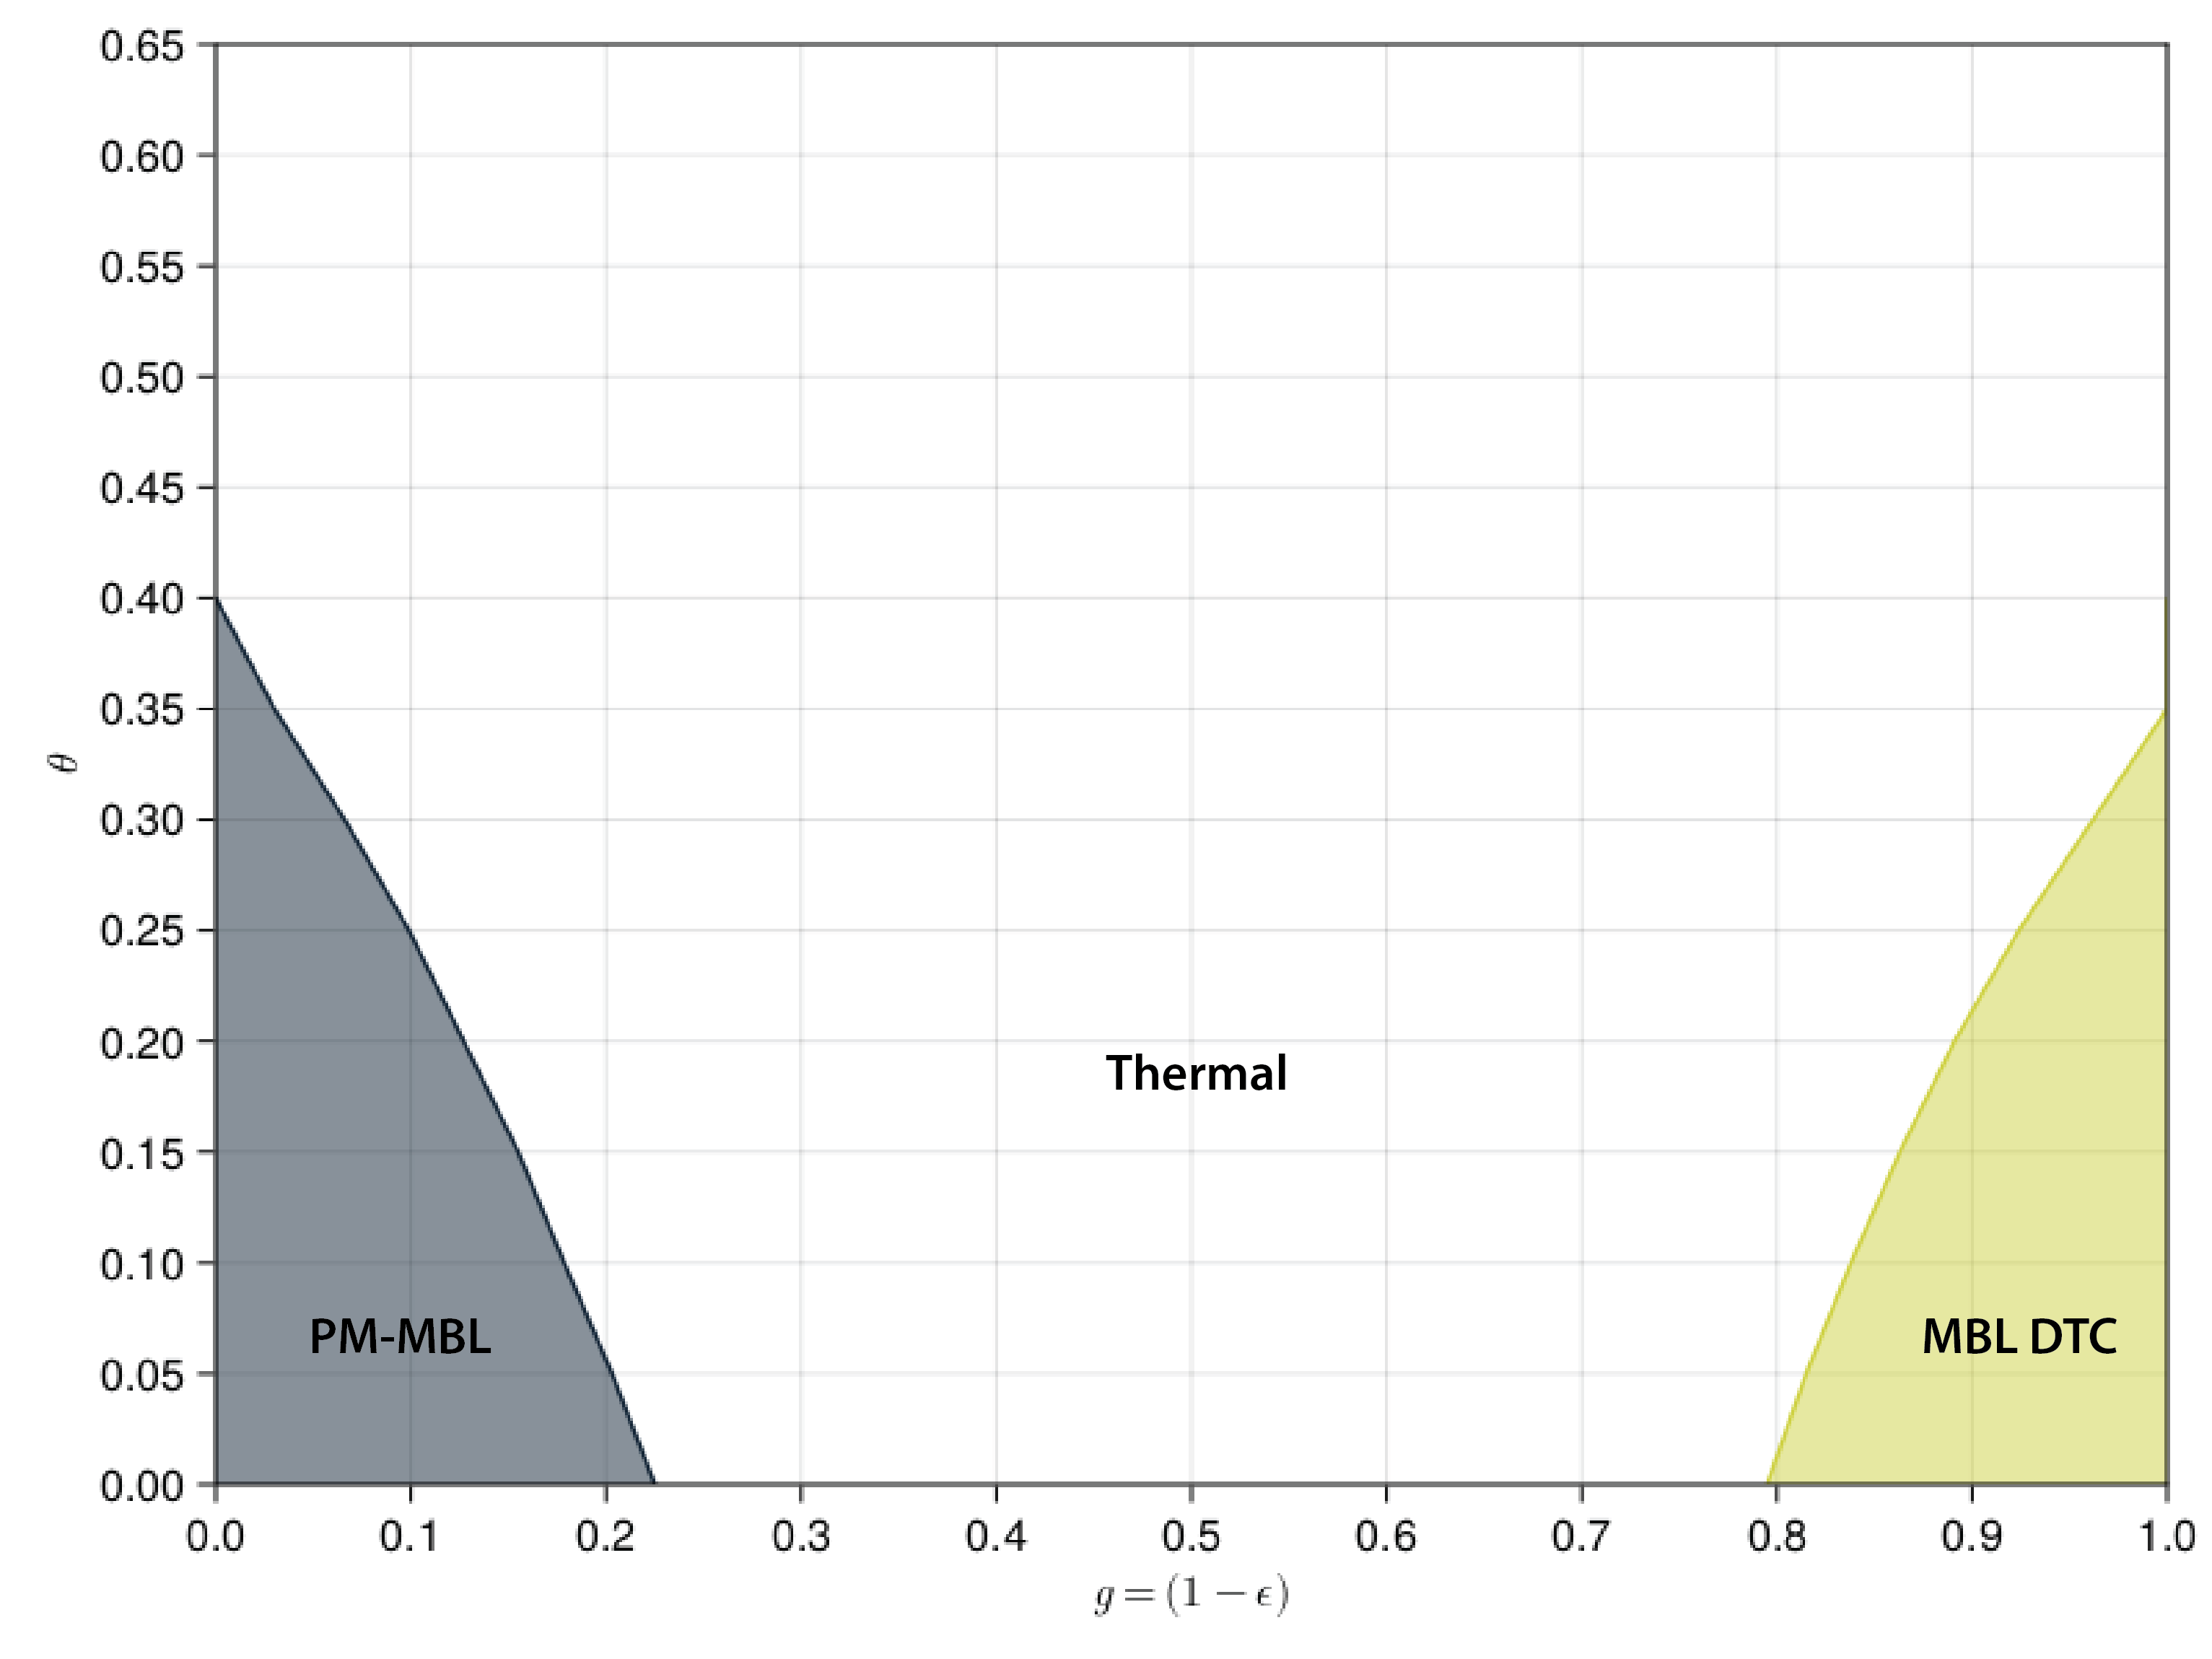
\includegraphics[width=0.9\linewidth]{.src/images/DTC/model/Phase_diagram_Labeled.png} 
\label{fig:DTC-phase-diagram}
\end{subfigure}
\caption{Schematic representation of the circuit and the associated phase diagram. The circuit exhibit three phases. For smaller values of $\theta$ and $\epsilon$ close to 1, that is $g$ close to 0, it can support a MBL phase which is paramagnetic in nature. For small $\theta$ and $\epsilon$ close to 0, that is $g$ close to 1, it supports a DTC MBL phase with a period multiplicity of 2. In the middle region the system tend to scramble. The phase boundary was extracted from results of \cite{Vedika2021DTCinNISQ}, and was obtained from finite size scaling of the disorder averaged level spacing ratio.} 
\label{fig:DTC-circuit-phase-diagram}
\end{figure}

The model we will be concerned with is the brick-wall circuit from Ipolitti et al \cite{Vedika2021DTCinNISQ,Ippolitti2022GoogleSycamore}. The General Floquet Model considered here, that exhibits a Discrete Time Crystal in 1D is an disordered Ising model with periodic $\pi/2$ Kicks about the $x$-axis. The system is probed only at stroboscopic times, $t=n \tau$, and $\tau=1$

\begin{equation}
    U_F= e^{-ig \pi\sum_i X_i}e^{-i\tau(\sum_{i} J_{i} Z_i Z_{i+1}+H_{int})}e^{-i\tau(\sum_{i} h_{i} Z_i)}
\end{equation}

Here we have adopted the standard information theoretic notation (i.e have denoted Pauli operator $\sigma^Z_i=Z_i$ etc.) The $H_{int}$ denotes some generic interaction such as fields or coupling, 

\begin{equation*}
\begin{split}
    H_{int}&=  \frac{\theta}{2}\sum_{i}[X_iX_{i+1}+Y_iY_{i+1}] \text{(XY Coupling)}
\end{split}
\end{equation*}


Among these parameters $J_i, h_i$ are disordered and are uniformly sampled from the following intervals  $J_i \in [0,\pi] , h_i \in [0,2\pi]$.  The disorder is utilised to ensure localisation and thereby to prevent the system from heating up to triviality from the kicks \cite{Vedika2015phasestructre}. Note that unlike the paramagnetic case, to stabilise time-crystalline MBL it is essential to have a disorder realisation on the Ising even couplings $J_i$, as otherwise the kicks cancels out the local background field over even periods (especially for small $\epsilon$, and exactly at the perfect time-crystalline point) \cite{Vedika2021DTCinNISQ}. The parameter $g=(1 - \epsilon)$ controls the angle of the kick and forms one of the tuning parameters.


We also add further small uncertainties in the realisations of the two body gates 

\begin{equation}
    \theta=[\Bar{\theta}-\frac{\Delta\theta}{2},\Bar{\theta}+\frac{\Delta\theta}{2}]
\end{equation}

where $\Delta\theta=\frac{\pi}{50}$ and random independently drawn small single body rotation noise to each $Z$ legs $j$ of each gates $i$, $RZ(\delta h_j)$, where $\delta h_j \in \mathcal{N}(0,\frac{\pi}{50})$.


In absence of interaction and with perfect kicks it is trivial to see that operators of the form $\braket{Z(0),Z(n)}$ breaks the discrete time symmetry and exhibits a period doubling. The non-triviality of the DTC as a \textit{phase} comes from the fact that this feature persists strongly even in the presence of interactions as well as with imperfect kicks (i.e $g=\frac{1}{2}=(\pi-\epsilon)$ with finite but small $\epsilon$). In a quantum device this is realised as a brick-wall circuit. Below we quote two images from \cite{Ippolitti2022GoogleSycamore} that simulated portions of this circuits on a 20 qubit 1-D subsystem of the Google Sycamore processor. Other later experiments include \cite{Frey2022IBMrealization} on 57 qubits of IBM Heron processor and exhibits similar results.


\begin{figure}[h!]
\centering
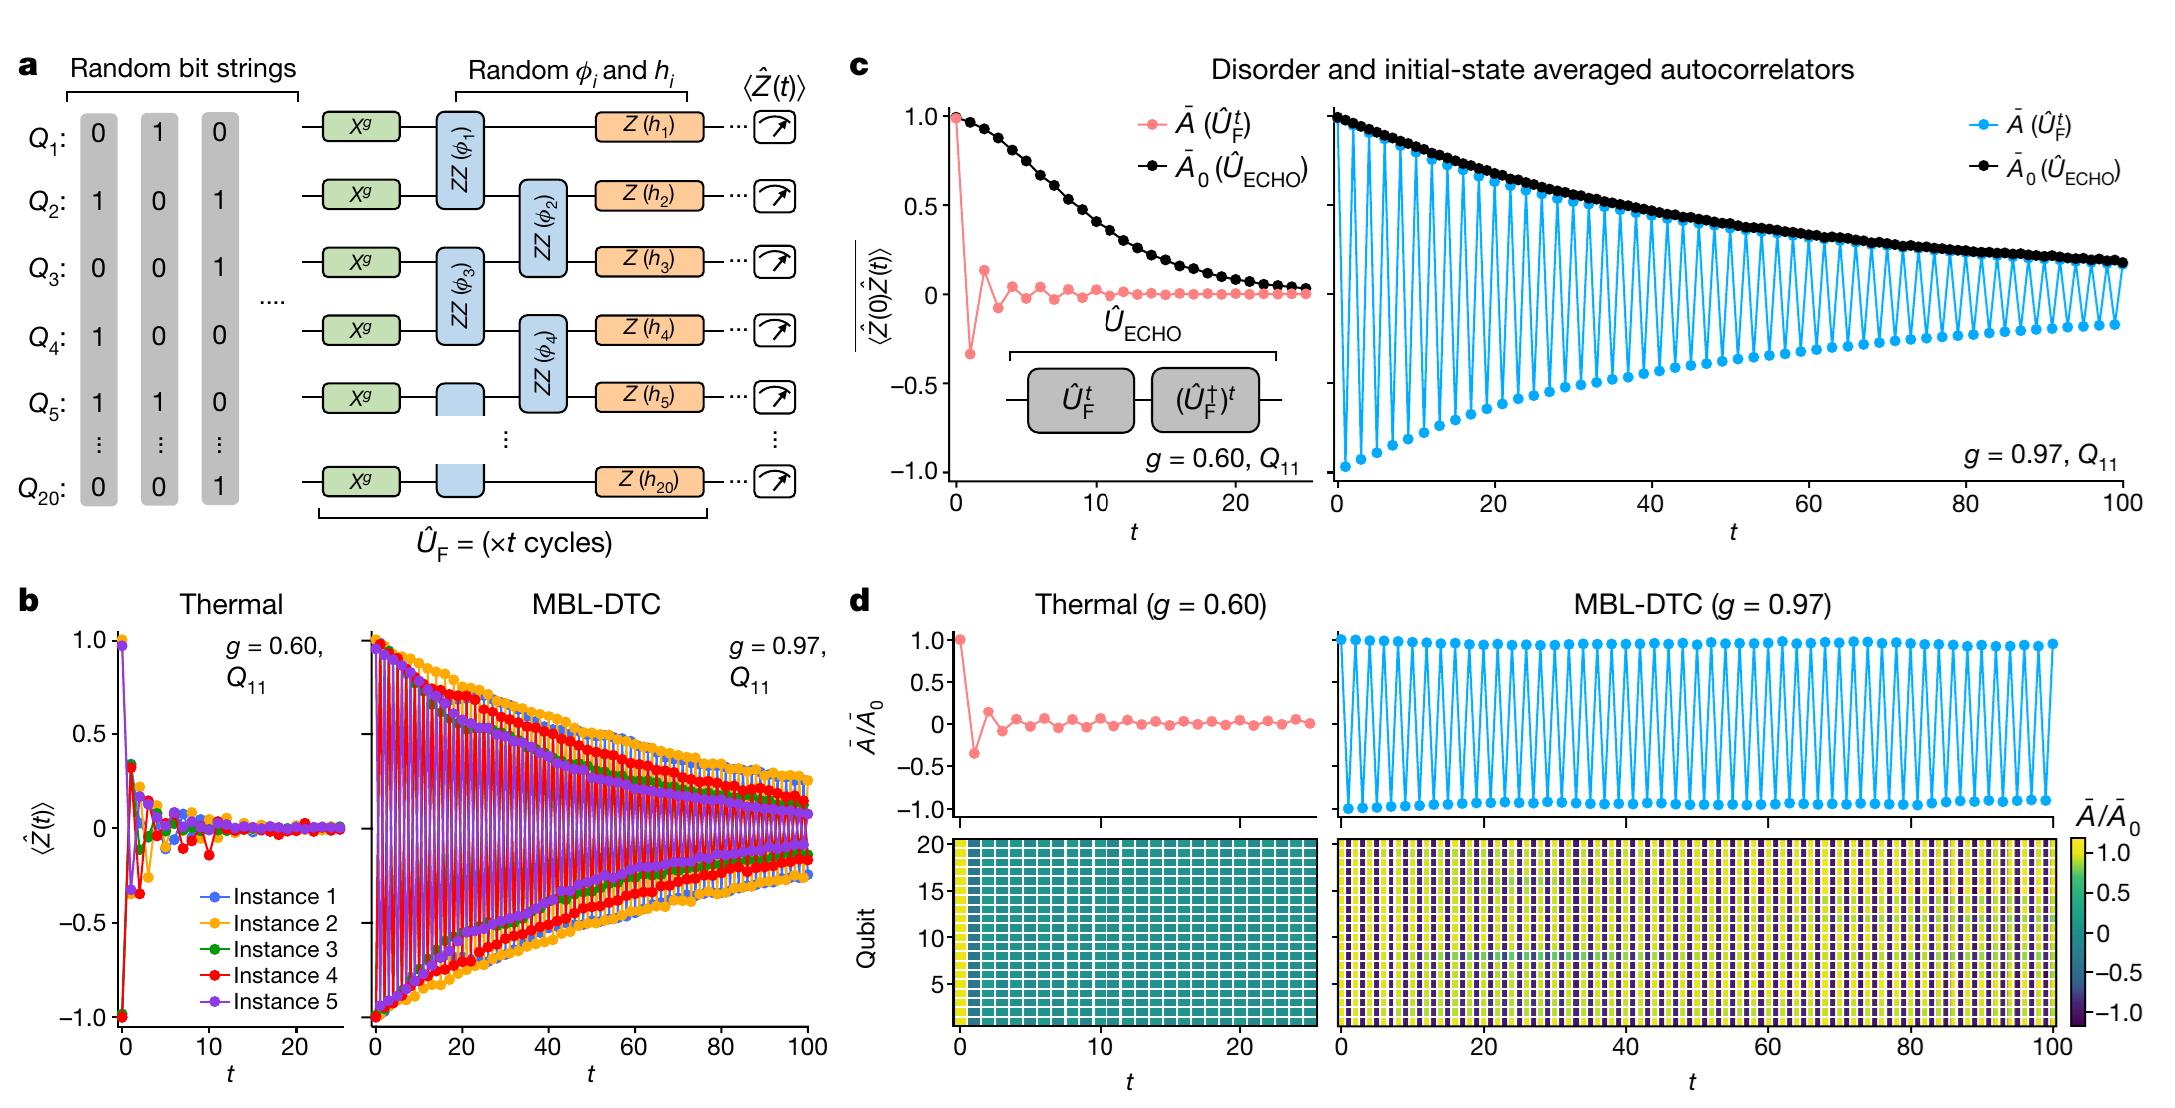
\includegraphics[width=\linewidth]{.src/images/DTC/model/ippolitti-experiment-on-sycamore-1.png}
\caption{
\textbf{Observing an MBL-DTC.}
(a) The experimental circuit composed of $t$ identical cycles of the unitary $\hat{U}_F$. 
The local polarization of each qubit, $\langle \hat{Z}(t) \rangle$, is measured at the end. 
In the following panels, we investigate a number of disorder instances each with a different random bit-string initial state. 
(b) Experimental values of $\langle \hat{Z}(t) \rangle$ measured at $Q_{11}$. 
Data are shown for five representative circuit instances deep in the thermal ($g = 0.60$; left) and MBL-DTC ($g = 0.97$; right) phases. 
(c) Autocorrelator $\overline{A} = \langle \hat{Z}(0)\hat{Z}(t) \rangle$ at $Q_{11}$, obtained from averaging the results of 36 circuit instances. 
For the same circuit instances, the average autocorrelator at the output of 
$\hat{U}_{\mathrm{ECHO}} = (\hat{U}_F^{\dagger})^t \hat{U}_F^t$ is also measured and its square root, $\overline{A}_0$, is shown alongside $\overline{A}$ for comparison. 
The left (right) panels correspond to $g = 0.60$ ($0.97$). 
(d) Top panels: the ratio $\overline{A}/\overline{A}_0$ obtained from (c). 
Bottom panels: $\overline{A}/\overline{A}_0$ as a function of $t$ and qubit location. 
The left (right) panels correspond to $g = 0.60$ ($0.97$).
}
\label{fig:MBL-DTC}
\end{figure}


\begin{figure}[t]
\centering
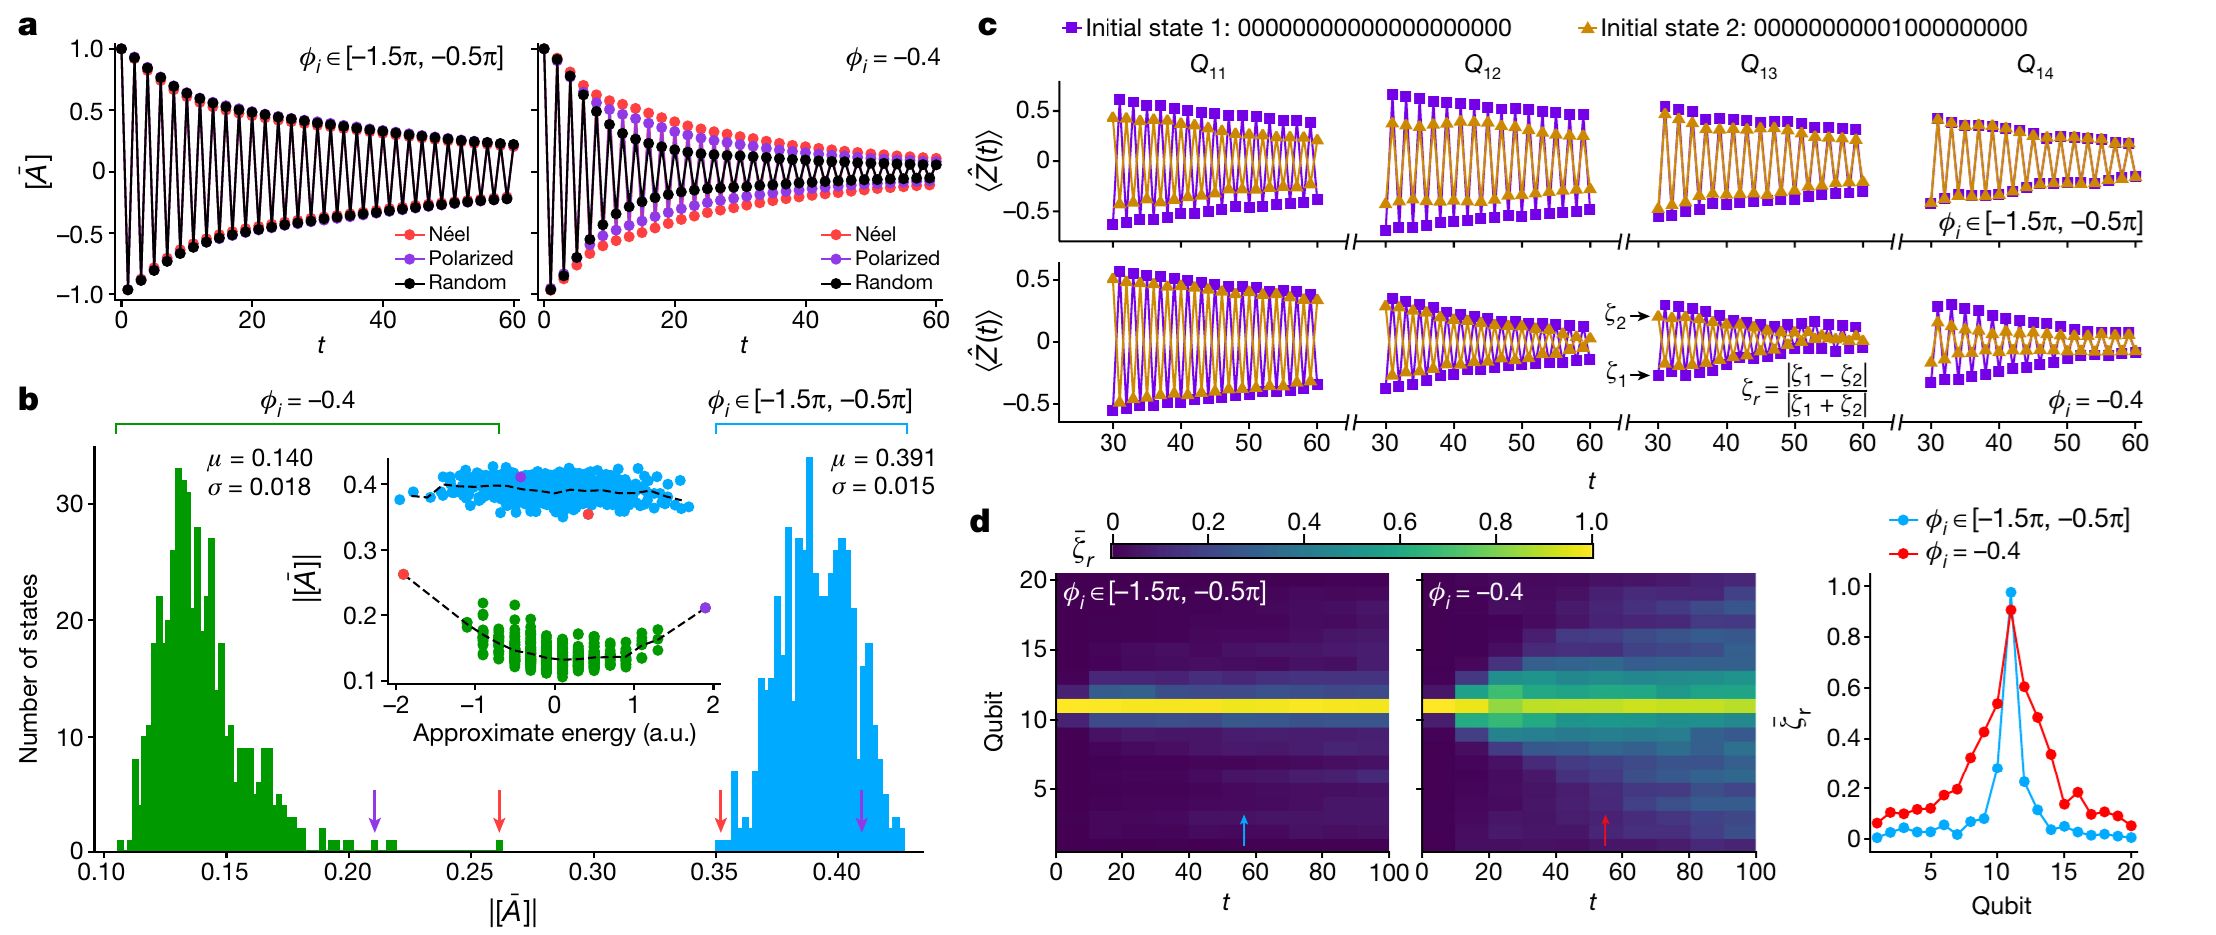
\includegraphics[width=\linewidth]{.src/images/DTC/model/ippolitti-experiment-on-sycamore-2.png}
\caption{
\textbf{Distinguishing MBL-DTC from prethermal phenomena.}
(a) Site- and disorder-averaged autocorrelators $\overline{A}$ measured with $g = 0.94$. 
In the left panel (MBL-DTC), each dataset is averaged over 24 disorder instances of $\phi_i$ and $h_i$, 
with the initial state fixed at one of the following: N\'eel, $\lvert 01 \rangle^{\otimes 10}$; polarized, $\lvert 0 \rangle^{\otimes 20}$; random, $\lvert 00111000010011001111 \rangle$. 
In the right panel (prethermal), the same values of $h_i$ and initial states are used but $g_i = -0.4$. 
(b) Histograms of $\lvert \overline{A} \rvert$, from 500 random bit-string initial states, averaged over cycles 30 and 31 and the same disorder instances as in (a). 
The standard deviation (mean) of $\lvert \overline{A} \rvert$, $\sigma$ ($\mu$), is also listed. 
Location of the polarized (N\'eel) state is indicated by a purple (red) arrow. 
\textit{Inset:} same collection of $\lvert \overline{A} \rvert$ plotted over the energies of the bit-string states, 
calculated from the effective Hamiltonian $\hat{H}_{\mathrm{eff}}$ approximating the drive (see text). 
Dashed lines show averaged values within energy windows separated by 0.2. 
(c) $\langle \hat{Z}(t) \rangle$ for two bit-string initial states that differ only at $Q_{11}$. 
Top panel shows a single circuit instance with disordered $\phi_i$, and bottom panel shows an instance with uniform $\phi_i = -0.4$. 
(d) Left and middle panels: relative difference between the two signals $\zeta_r$ as a function of $t$ and qubit location, 
averaged over time windows of 10 cycles and over 64 disorder instances for $\hat{U}_F$ and 81 instances for $\hat{U}_F$. 
Right panel: qubit dependence of $\zeta_r$, averaged from $t = 51$ to $t = 60$.
}
\label{fig:MBL-DTC-distinction}
\end{figure}
